\documentclass[french,a4paper,12pt]{report}
\usepackage[utf8]{inputenc}
\usepackage[T1]{fontenc}
\usepackage{graphicx}
\usepackage{float}
\usepackage{listings}
\usepackage{color}
\definecolor{dkgreen}{rgb}{0,0.6,0}
\definecolor{gray}{rgb}{0.5,0.5,0.5}
\definecolor{mauve}{rgb}{0.58,0,0.82}

\lstset{frame=tb,
  language=Java,
  aboveskip=3mm,
  belowskip=3mm,
  showstringspaces=false,
  columns=flexible,
  basicstyle={\small\ttfamily},
  numbers=none,
  numberstyle=\tiny\color{gray},
  keywordstyle=\color{blue},
  commentstyle=\color{dkgreen},
  stringstyle=\color{mauve},
  breaklines=true,
  breakatwhitespace=true,
  tabsize=3
}



\title{LO52\\ Travaux Pratiques 2 :\\ Introduction à l'AOSP}
\author{Professeur encadrant : BRISSET Fabien \\ Elèves : \\ROMET Pierre
\\PROST Guillaume \\ \\ \\}
\date{Automne 2017}

\begin{document}

\begin{document}

\maketitle
\tableofcontents

\chapter{Objectifs}
Lors de ce tp, deux principaux objectif nous furent fixé.
Le premier concernait la mise en place du modèle de données pour la gestion des volants.
Le second fut de développer une application intégrant le modèle de données.

\section{Application de gestion des volants}
\subsection{4.1}
En nous référent à l'énoncé du tp, afin de rendre notre développement d''application
le plus proche possible d'un cas réelle, il nous fut proposé de reprendre l'identité
d'un des plus gros revendeur de volant français, "LardeSports".
En conséquence, nous avons du modifier le titre de nos activités afin que celui-ci
affiche "LardeSports".

Pour cela, nous avons du créer une nouvelle entrée "String" dans le fichier "strings.xml"

\begin{lstlisting}
    <string name="app_name">LardeSports</string>
\end{lstlisting}

Puis, dans le fichier "AndroidManifest.xml" (se trouvant dans le dossier Manisfest),
il ne nous reste plus qu'à attribuer la STRING "app_name" à la variable:

\begin{lstlisting}
    android:label="@string/app_name"
\end{lstlisting}

Grâce à cette mécanique, il nous est possible de créer des variables d'envirronment,
aisément réutilisable, toutes contenus au sein du même fichier "strings.xml".

Par la suite, il nous fut demandé de d'implémenter de nouvelles activitées "Achats"
et "Stock", devant toutes deux être accécible depuis l'activité principale.

Pour cela, nous avons commencé par ajouter deux boutons, "ACHAT" et "STOCK", où pour
chacun, nous avons lié une fonction via la propriété "onClick()" (attribut permettant
de déclancher une fonction par une pression sur l'élément définie).

\subsection{4.2: Composition de l’activité}

Pour afficher la liste des produits en stock, nous avons utilisé une activité vide,
 dans laquelle nous avons placé une liste (composant ListView).

 \subsection{4.3: Cellules personnalisées de la liste}
 La complexité de cette nouvelle activité vient principalement de la structure
 particulière des cellules. En effet, dans les cellules de cette liste, il fallait
 afficher diverses informations à propos du produit correspondant à la ligne :
 le nom de la marque, la référence du produit, le prix, le nombre de produits en
 stock et un visuel du produit.

 \hfill\hbox to 0pt{\hss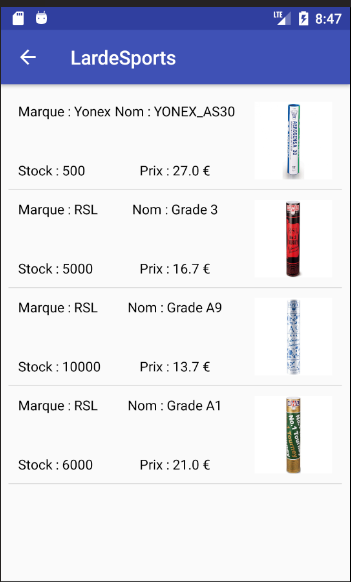
\includegraphics[width=7cm]{Rapport_screen_activity-Stock_liste.png}\hss}\hfill\null\newline

Pour réaliser le layout spécifique de la liste, nous avons créé deux composants.
Le premier est un fichier de layout pour décrire la structure d’une cellule via
un simple fichier XML. Chacun des éléments mentionnés ci-dessus a donc un élément
graphique décrit ici. Les positions de chacun sont relatives au parent de ces éléments,
c’est-à-dire le layout de la cellule. Ces positions ne sont pas définies les unes
 par rapport aux autres, et il se peut que les différents éléments soient superposés
 dans certains cas. Cependant, dans notre cas et pour cette activité-ci, aucune des
 données n’est suffisamment longue pour provoquer une telle situation, aussi avons
 choisit de ne pas modifier outre mesure ce layout pour le moment.
Enfin, le deuxième élément qu’il nous a fallu créer est une classe java permettant
d’associer les données de notre produit aux différents composants graphiques Android
que nous avons décrit dans le fichier XML de layout. Pour des raisons de simplicité,
cette classe hérite de la classe ArrayAdapter, fournie par Android, qui est généralement
utilisée pour faire ce genre de mapping entre données et interface.
Cette classe possède en interne un holder contenant les instances des composants
graphiques, et surcharge la méthode getView(…), qui est appelée lorsque l’interface
 doit être mise à jour. C’est dans cette méthode que les données du produit vont
 être données aux composants graphiques.

\subsection{4.5}
Comme vu dans la partie "4.1", il nous faut maintenant implémenter les fonctions
appelés par l'évènement "onclick()".
Ces fonctions sont composées d'un "INTENT"; object permettant de lier deux entitées
distinctes tels que des activitées, l'INTENT représentant la capacité d'une activiter
à faire quelque chose. Ici, nous l'utilisons afin de lancer une activité secondaire
à partir de notre activité principale.

Le constructeur de notre INTENT prend deux paramètres:
\begin{itemize}
  \item Contexte:
  Nécessaire car une "Activity" Class is a subclass of Context
  \item Classe:
  La classe de l'application composante envert laquelle le système doit delivrer
  l'INTENT.
\end{itemize}

\begin{lstlisting}
/** Called when the user taps the Send button */
public void AchatSend(View view) {
    Intent intent = new Intent(this, Achats.class);
    startActivity(intent);
}
\end{lstlisting}

Enfin, une fois arrivé dans notre activité secondaire, suite au lancement effectué
au sein de l'activité principale, il nous faut mettre en place une mécanique afin de
pouvoir revenir sur notre activité parente. Pour cela, avons mis en place une flèche
de navigation au sein de l'"app bar".
Pour cela, il nous a simplement fallu définir une activité parent logique, pour chacune
de nos activitées secondaire, au travers du fichier "AndroidManifest.xml".

Par exemple, pour l'activité secondaire "Achat", la classe parente sera la classe
".MainActivity".
\begin{lstlisting}
<activity
          android:name=".Achats"
          android:parentActivityName=".MainActivity">
          <meta-data
              android:name="android.support.PARENT_ACTIVITY"
              android:value=".MainActivity" />
      </activity>
\end{lstlisting}

\subsection{4.6}
Pour finir, au sein de l'activité "Achat", il nous faut maintenant pouvoir lister
pour chaque achats:
\begin{itemize}
  \item Un/une acheteur/acheteuse
  \item Un prix
  \item Une quantité
  \item Une référence
  \item Le tout affiché en vert si c'est payé, en rouge sinon
\end{itemize}

Dans un premiers temps, afin de pouvoir effectuer un listening de tous les achats
effectué, nous avons mise en place un objet "ListView" afin de disposer, pour chaque
achat, de toutes les données souhaité, présenté ci-dessus.
Au sein de cette "ListView", chaque données sera représenté de la manière suivante:

\begin{lstlisting}
<TextView
  android:id="@+id/buyer"
  android:layout_width="wrap_content"
  android:layout_height="wrap_content"
  android:textAppearance="?android:attr/textAppearanceSmall"
  android:textColor="@android:color/black" />
\end{lstlisting}

Chacune, disposera d'un identifiant, permettant d'identifier la donnée.
De valeur de positionnement, d'apparance, et de couleur.

Ensuite, il nous a fallu pouvoir, via un setter, fournir des informations à ces données
(acheteur, prix, etc...), pour cela, nous avons utilisé une classe "Databean", pouvant
contenir chacune de ces informations, puis nous en avons fais une liste.

\begin{lstlisting}
dataModels = new ArrayList<>();
//TODO Utiliser la BDD pour gather les données (passer par une classe de DAO)
dataModels.add(new AchatDataBean("Yonex", "YONEX_AS30", 27.0, 500, R.drawable.yonex_as30));
dataModels.add(new AchatDataBean("RSL", "Grade 3", 16.7, 5000, R.drawable.rsl_grade_a3));
dataModels.add(new AchatDataBean("RSL", "Grade A9", 13.7, 10000, R.drawable.rsl_grade_a9));
dataModels.add(new AchatDataBean("RSL", "Grade A1", 21.0, 6000, R.drawable.rsl_grade_a1));
\end{lstlisting}

Ainsi, chacune des informations peuvent être ajuter à loisir en fonction du besoin et des
actions effectué au sein de l'appli.

La dernière partie reste la classe "achat_CustomAdapter", nous permettant de mettre à jours
le visuel de notre appli.
Via le constructeur de notre classe, nos données sont connecté à notre "ListView", qui au travers
d'un getter va pouvoir récupérer différentes données (acheteur, prix, etc...), et les setter
aux différents éléments graphiques en présence, comme le montre
le code ci-dessous.

\begin{lstlisting}
viewHolder.buyerTxtView.setText(String.format("Acheteur : %s",StockDataBean.getBuyer()));
viewHolder.referenceTxtView.setText(String.format("Référence : %s",StockDataBean.getReference()));
viewHolder.priceTxtView.setText(String.format("Prix : %s €",Double.toString(StockDataBean.getPrice())));
viewHolder.quantityTxtView.setText(String.format("Quantité : %s",Integer.toString(StockDataBean.getQuantity())));
viewHolder.overviewImgView.setImageResource(StockDataBean.getOverviewImgRes());
\end{lstlisting}

Pour finir,
La couleur devant permettre de savoir si un achat à été réglé ou non (vert -> payé,
rouge -> non payé) sera implémenté au travers de l'attribut "textColor" des items
de "ListView", comme le montre le code ci dessous:

\begin{lstlisting}
<TextView
  android:id="@+id/buyer"
    android:textColor="@color/green"
  android:layout_width="wrap_content"
  android:layout_height="wrap_content"
  android:textAppearance="?android:attr/textAppearanceSmall"
  android:textColor="@android:color/black" />
\end{lstlisting}

\chapter{Application de gestion de volants - Advanced Mode}

\section{Modèle de l’activité}
Concernant le stockage des données de nos produits, nous avons créé une classe
StockDataBean suivant la structure d’un bean pour mémoriser les données des produits.
Pour mémoriser les images qui correspondent aux visuels des produits, nous avons
ajouté un attribut de type int à cette classe, puisque les références vers des
images ressources sont des variables de type int sous Android.
Nous avons également ajouté les visuels des produits aux ressources de notre projet,
 dans le dossier app\src\main\res\drawable-mdpi. Au niveau du code Java, la récupération
 des références vers ces images ressources se fait via la formule suivante :
 R.drawable.<nom_de_l_image>.

 \section{Détail d’une commande}
Dans la partie 5 de ce TP2, il nous a été demandé de faire une nouvelle activité
(nommée ShuttleOrderActivity dans notre projet) permettant de visualiser une commande.
Nous avons décidé que cette activité serait accessible depuis un bouton présent dans
le menu principal, arrivant sur l’activité vide de données pour composer une nouvelle
commande, tout en ayant bien sûr l’accès via l’activité de stock, accès arrivant
cette fois-ci sur une version pré-remplie de l’activité de commande, comme demandé
dans l’énoncé.

\section{Composition de l’activité}
L’interface de cette activité se présente comme il suit :

\hfill\hbox to 0pt{\hss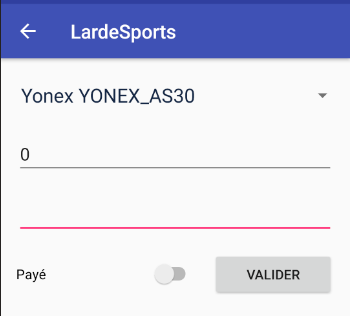
\includegraphics[width=7cm]{Rapport_screen_activity-ShuttleOrder_gui_spinner_collapsed.png}\hss}\hfill\null\newline

\hfill\hbox to 0pt{\hss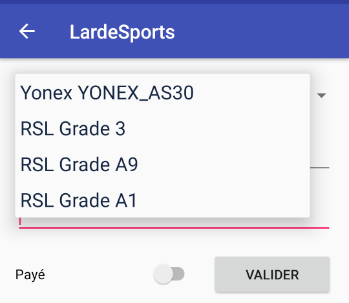
\includegraphics[width=7cm]{Rapport_screen_activity-ShuttleOrder_gui_spinner_expanded.png}\hss}\hfill\null\newline

Tout d’abord, nous avons un champ de type Spinner, permettant de sélectionner
le produit associé à la commande. Nous avons choisi le Spinner parce que ce
composant nous permet d’avoir un menu déroulant, affichant ainsi la liste des
produits disponibles. L’autre choix possible, que nous avons rejeté, était le
champ texte avec auto-complétion. Nous l’avons rejeté, car un composant de ce
type nécessite de connaître à l’avance le nom du produit, alors que le Spinner
offre la possibilité de parcourir dans une certaine mesure le catalogue de produits.
Nous avons égalements des champs texte et nombres classiques pour le nombre de
produits et le nom de l’acheteur. Le dernier composant est un simple switch à deux
 positions représentant l’état Payé/Non-payé.

L’une des contraintes de cette activité était de pouvoir spécifier un id de commandes,
 qui servirait à remplir les champs à l’affichage de l’activité. Dans ce cas de figure,
 nous devions verrouiller les champs de saisie, ne permettant à l’utilisateur de modifier
 que le switch.
Nous avons réussi à obtenir un comportement de ce type en utilisant un extra dans
l’objet Intent lançant l’activité. Si un extra est présent dans l’intent, sa valeur
est utilisée pour récupérer une commande dans la base de données (ou dans les données
en brut). Si une commande peut être récupérée par cette méthode, l’activité se lance
donc dans le mode « restreint », avec les champs verrouillés et pré-remplis. Si aucune
commande ne peut être récupérée ou si l’extra n’est pas présent dans l’intent, alors
l’activité se lance en mode « libre », avec les champs modifiables et vides.

\hfill\hbox to 0pt{\hss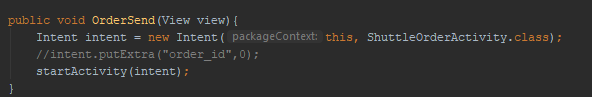
\includegraphics[width=12cm]{Rapport_screen_activity-MainActivity_intent_order.png}\hss}\hfill\null\newline

Sur la capture ci-dessus, nous pouvons voir un exemple de lancement d’Intent permettant
d’afficher notre activité. En commentaire se trouve la ligne permettant d’ajouter le
paramètre spécifiant l’identifiant de la commande à utiliser pour pré-remplir les champs
(sur l’image, cet identifiant est 0).

Nous avons paramétré l’activité pour que le parent de celle-ci soit l’activité MainActivity.
À terme, ce paramétrage sera modifié pour que le bouton « back » amène vers l’activité ayant
lancé l’Intent initial, de manière à avoir un véritable comportement de bouton « retour arrière ».

\section{Modèle de l’activité}
En interne, nous utilisons notre classe StockDataBean pour les données du produit,
ainsi qu’une nouvelle classe de type bean nommée OrderDataBean, contenant les données
de la commande. Ce bean ne contient aucune données relatives à un produit à l’exception
de l’identifiant. Ce système nous permettra un minimum de modifications dans le code de
ces classes lorsque l’implémentation d’une base de données SQLite sera faite.
La totalité de la liste des produits est chargée dans l’activité, pour remplir le
menu déroulant du composant Spinner. La liste des commandes est également chargée,
mais à terme, avec l’utilisation d’une base de données SQLite, seule la commande
correspondante à l’id fourni (dans le cas de figure où un extra est donné à l’intent)
sera chargée.

\section{Base de donnée SQLite}
Dernier élément demandé lors de ce TP, une base de données SQLite permettant de
stocker et récupérer les produits et les commandes.
Pour ce faire, nous avons réutilisé le principe que nous avions testé lors du TP1,
à savoir la classe DataBaseHelper, qui permet de générer un objet SQLiteDatabase,
avec lequel nous pouvons par la suite effectuer des requêtes SQL pour manipuler notre BDD.
La principale différence dans cette classe par rapport au TP1 est que nous avons
créé en dur les tables et les données, au lieu d’utiliser un fichier .sql pour cela.
La structure des tables a également été simplifiée pour n’avoir que deux tables,
Table\_shuttle et Table\_order, dont les champs correspondent aux attributs de nos
 classes xxxDataBean décrit précédemment.
Malheureusement, nous n’avons pas réussi à créer les tables via cette méthode,
la base de données étant montée avec succès, mais restant vide malgré les requêtes
de création.

En plus de cette classe DataBaseHelper, nous avons créé deux classes de DAO,
une pour le stock (SQLiteStockDao) et une pour les commandes (SQLiteOrderDao),
encapsulant la gestion des accès à la base de données. Ces classes ont toutes
les deux des interfaces qu’elles vont implémenter (respectivement IStockDao et
IOrderDao), nous permettant ainsi de changer l’implémentation en runtime (très
utile lors des phases de test des interfaces).
Ces classes de DAO ont été utilisées dans l’activité ShuttleOrderActivity pour
les phases de tests de la BDD, mais étant donné que la mise en place actuelle
ne permet pas son utilisation, aucune des autres activités n’utilisent les DAO.








\end{document}
